% Fig. 4.6 -- 三條卡方密度曲線疊在同一組座標軸上，自由度依序為 10、20、30。
% 書稿來源: mathstatch4.tex 第 3951 至 3980 行的 tikzpicture (pgfplots 的 axis 環境，
%   width=.8\textwidth、height=.5\textwidth)。
%
% 書稿以 declare function 定義 eee(k,a,b) = (1/(b^a (a-1)!)) k^(a-1) e^{-k/b}，
% 也就是形狀參數為整數的伽瑪密度，三條曲線取 (a,b) = (5,2)、(10,2)、(15,2)，
% 即自由度 nu = 2a = 10、20、30 的卡方密度; 本檔直接寫成卡方的形式
%   f(x) = x^{nu/2-1} e^{-x/2} / (2^{nu/2} Gamma(nu/2))
% 兩者是同一個函數。
%
% 數值寫法: 直接以 x^{nu/2-1} 作圖會讓 pgfmath 溢位 (nu=30 時 x^14 在 x=65 之下
%   達 1.3e25，pgfmath 的定點數上限只有 16383.99998)，故改寫為以眾數 m = nu-2
%   為基準的相對式
%     f(x) = f(m) * exp( a * ln(x/m) - (x-m)/2 ),  a = nu/2-1
%   指數項一律為非正數，不會溢位，也避免了大數相減的失真。三個峰值 f(m) 由
%   lgamma 另行算出並寫死在下面:
%     nu=10: a=4,  m=8,  f(m)=0.0976834
%     nu=20: a=9,  m=18, f(m)=0.0658778
%     nu=30: a=14, m=28, f(m)=0.0529946
%   實測 pgfmath 與 Python 的 lgamma 版本在峰頂與各刻度處相差不到千分之二。
%
% 對書稿的三處調整:
%   1. 線型: 書稿為實線、dotted、dashed，本檔依 CH2_FIGURE_SPECS 1.9 節固定的
%      三種線型改為實線、on 1pt off 2pt、on 4pt off 2pt，對應關係不變
%      (nu=10 實線、nu=20 點線、nu=30 虛線)，一律 journalink，不以顏色分辨。
%   2. 標示: 書稿用 pgfplots 的 legend，本檔依同節「標註優先直接寫在曲線上」
%      改為把 $\nu=10$、$\nu=20$、$\nu=30$ 各寫在該曲線的峰頂正上方 0.19cm 處。
%      三個峰彼此相距 10 個單位，其餘兩條曲線在該處的高度都不到峰高的四分之一，
%      標示不會指向錯的曲線。
%   3. 書稿設了 ylabel 為 $f_X(x)$，但同時設 axis y line=none，實際上不會顯示，
%      本檔一併不畫縱軸與縱軸名。
%
% 座標: x 由 -0.5 到 66、刻度 0,10,...,60 (照書稿)，y 由 0 到 0.12 (照書稿)。
%   x=0.115cm、y=40cm，繪圖範圍 7.65cm 寬、4.80cm 高，寬高比 0.628，
%   與書稿的 .8:.5 = 0.625 相當。
%
% 產製:
%   pdflatex chi-square-density-family.tex
%   pdftocairo -svg chi-square-density-family.pdf \
%     ../../images/teaching-topics/chi-square-density-family.svg

\documentclass[tikz,border=2pt]{standalone}
\usepackage{amsmath}
\usepackage{amssymb}
\usepackage{xcolor}
\usetikzlibrary{arrows.meta}

%% 圖內沒有下標，最小字即 10pt 的內文級。
\DeclareMathSizes{10}{10}{9}{9}

\definecolor{journalink}{HTML}{1F1C18}
\definecolor{journalmuted}{HTML}{8A7F72}
\definecolor{journalaccent}{HTML}{9C2D2D}

\begin{document}
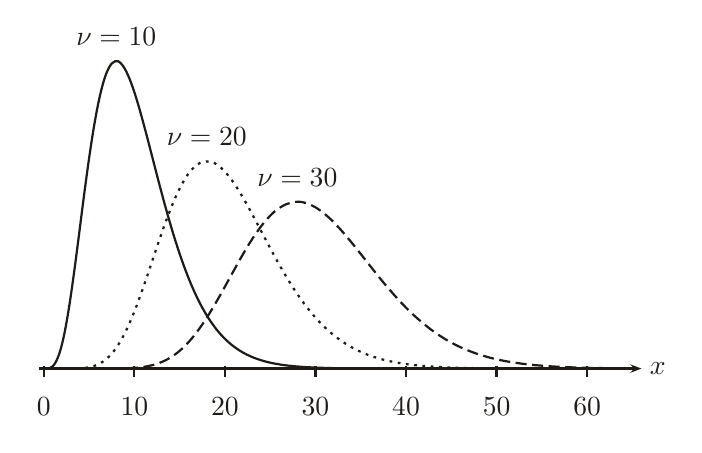
\begin{tikzpicture}[
  x=0.115cm,
  y=40cm,
  every node/.style={font=\normalsize, journalink},
  axis/.style={journalink, line width=0.8pt, -{Stealth[length=4pt]}},
  tick/.style={journalink, line width=0.8pt},
  curveten/.style={journalink, line width=0.8pt},
  curvetwenty/.style={journalink, line width=0.8pt,
                      dash pattern=on 1pt off 2pt},
  curvethirty/.style={journalink, line width=0.8pt,
                      dash pattern=on 4pt off 2pt}
]
  %% ---- 三條密度曲線 ------------------------------------------------------
  %% nu = 10: a = 4, 眾數 8, 峰值 0.0976834
  \draw[curveten] plot[domain=0.01:65, samples=200, smooth]
    (\x,{0.0976834*exp(4*ln(\x/8)-(\x-8)/2)});

  %% nu = 20: a = 9, 眾數 18, 峰值 0.0658778
  \draw[curvetwenty] plot[domain=0.01:65, samples=200, smooth]
    (\x,{0.0658778*exp(9*ln(\x/18)-(\x-18)/2)});

  %% nu = 30: a = 14, 眾數 28, 峰值 0.0529946
  \draw[curvethirty] plot[domain=0.01:65, samples=200, smooth]
    (\x,{0.0529946*exp(14*ln(\x/28)-(\x-28)/2)});

  %% ---- x 軸 --------------------------------------------------------------
  \draw[axis] (-0.5,0) -- (66,0);
  \node[anchor=west, inner sep=2.8pt] at (66,0) {$x$};

  \foreach \p in {0,10,20,30,40,50,60}
    \draw[tick] ([yshift=0.035cm]\p,0) -- ([yshift=-0.106cm]\p,0);
  \foreach \p in {0,10,20,30,40,50,60}
    \node[anchor=north] at ([yshift=-0.25cm]\p,0) {$\p$};

  %% ---- 三個自由度的標示，各寫在該曲線的峰頂正上方 ------------------------
  %% 峰頂之上 0.19cm (0.00475 個 y 單位) 處，anchor=south。
  \node[anchor=south, inner sep=0pt] at (8,0.1024)  {$\nu=10$};
  \node[anchor=south, inner sep=0pt] at (18,0.0706) {$\nu=20$};
  \node[anchor=south, inner sep=0pt] at (28,0.0577) {$\nu=30$};
\end{tikzpicture}
\end{document}
